\section{External interface requirements}
\label{sec:external_interface_requirements}%

\subsection{User interfaces}
\label{subsec:User_interfaces}%
The S\&C system will be a web app accessible by different devices and form factors, with a responsive UI. The UI will be different based on the type of user, reflecting the different functionalities they need. Every user will need to insert their credentials to have access to the platform and there will be a mechanism to recover them in case of a loss. The UI will comply with accessibility standards to ensure usability for all users, including those with disabilities.

\subsection{Hardware interfaces}
\label{subsec:hardware_interfaces}%
Our platform is a web app, as a consequence, it does not require any specific hardware
interface. Users only need a device with a browser to access the website and an internet connection. Latest versions of browsers are suggested to ensure compatibility and optimal performance. The user is free to choose his device but accessing the web app from a desktop form factor is strongly recommended for the best user experience.


\subsection{Software interfaces}
\label{subsec:software_interfaces}%
No specific software interfaces are needed. However, a mailing system to send confirmation emails will be used to the users during the registration process. In the future, integrations with university and company tools will be possible to enhance interoperability.

\subsection{Communication interfaces}
\label{subsec:communication_interfaces}%
The communication interfaces needed by the system include the HTTPS protocol for secure data transfer between the client and server. SSL/TLS certificates will ensure encrypted communication to protect user credentials and sensitive information.

\section{Functional requirements}
\label{sec:functional_requirements}%

\subsection{Requirements}
\label{subsec:requirements3}%
\newcounter{req}
\setcounter{req}{1}
\newcommand{\creq}{\thereq\stepcounter{req}}
\begin{center}
    \begin{longtable}{|l|p{0.9\linewidth}|}
        \hline
        \textbf{ID} & \textbf{Description}\\
        \hline
        R\creq & {The system allows STs to register by providing personal information, email, and a password.}\\
        \hline
        R\creq & {The system shall allow Users to log in using their credentials.}\\
        \hline
        R\creq & {The system shall allow STs to edit their profiles, including personal details and contact information.}\\
        \hline
        R\creq & {The system shall enforce role-based access control to restrict access to specific functionalities based on the user type (ST, CP, UV).}\\
        \hline
        R\creq & {The system shall allow CPs to post new internship opportunities, including position details, required skills, duration, and compensation.}\\
        \hline
        R\creq & {The system shall allow STs to apply for internships by submitting a CV and optional cover letter.}\\
        \hline
        R\creq & {The system shall notify CPs when STs apply to an internship.}\\
        \hline
        R\creq & {The system shall allow CPs to review applications and schedule interviews with STs.}\\
        \hline
        R\creq & {The system shall allow CPs to submit questionnaires to STs.}\\
        \hline
        R\creq & {The system shall allow CPs to accept or reject applications and notify STs of the decision.}\\
        \hline
        R\creq & {The system shall allow UVs to manage their students and monitor their activity.}\\
        \hline
        R\creq & {The system shall send notifications to users for events such as application submissions, approvals, or rejections.}\\
        \hline
        R\creq & {The system shall allow CPs to track the progress of STs during the internship and provide regular feedback.}\\
        \hline
        R\creq & {The system shall allow CPs to evaluate the performance of STs at the end of the internship.}\\
        \hline
        R\creq & {The system shall allow UVs to review the feedback and evaluation provided by both CPs and STs.}\\
        \hline
        R\creq & {The system shall allow STs to search for internships using keywords, filters, or location.}\\
        \hline
        R\creq & {The system shall recommend internships to STs based on their skills, preferences, and past applications.}\\
        \hline
        R\creq & {The system shall recommend STs to CPs for specific internships based on their skills, preferences, and past applications.}\\
        \hline
        R\creq & {The system shall allow CPs to search for suitable STs based on their skills, academic background, and CVs.}\\
        \hline
        R\creq & {The system shall maintain a database of all internships, applications, and evaluations.}\\
        \hline
        \caption{Requirements.}
        \label{tab: requirements}%
    \end{longtable}
\end{center}

\subsection{Use case diagrams}
\label{subsec:use_case_diagrams}%

\begin{figure}[H]
    \begin{center}
        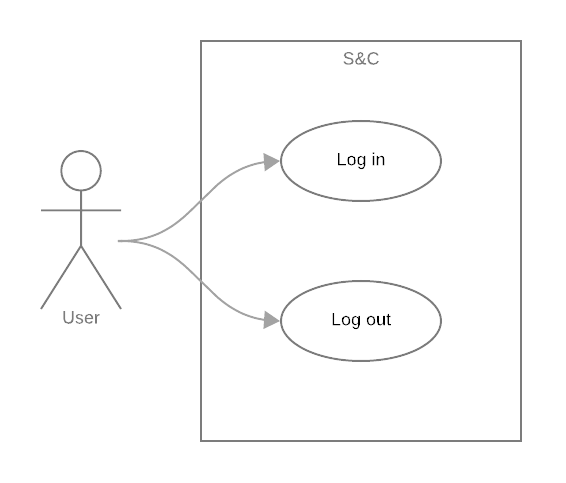
\includegraphics[width=0.8\linewidth]{UseCaseDiagrams/UC_User.png}
        \caption{Use Cases Diagram for all users.} 
        \label{fig:UserUC}%
    \end{center}
\end{figure}

\begin{figure}[H]
    \begin{center}
        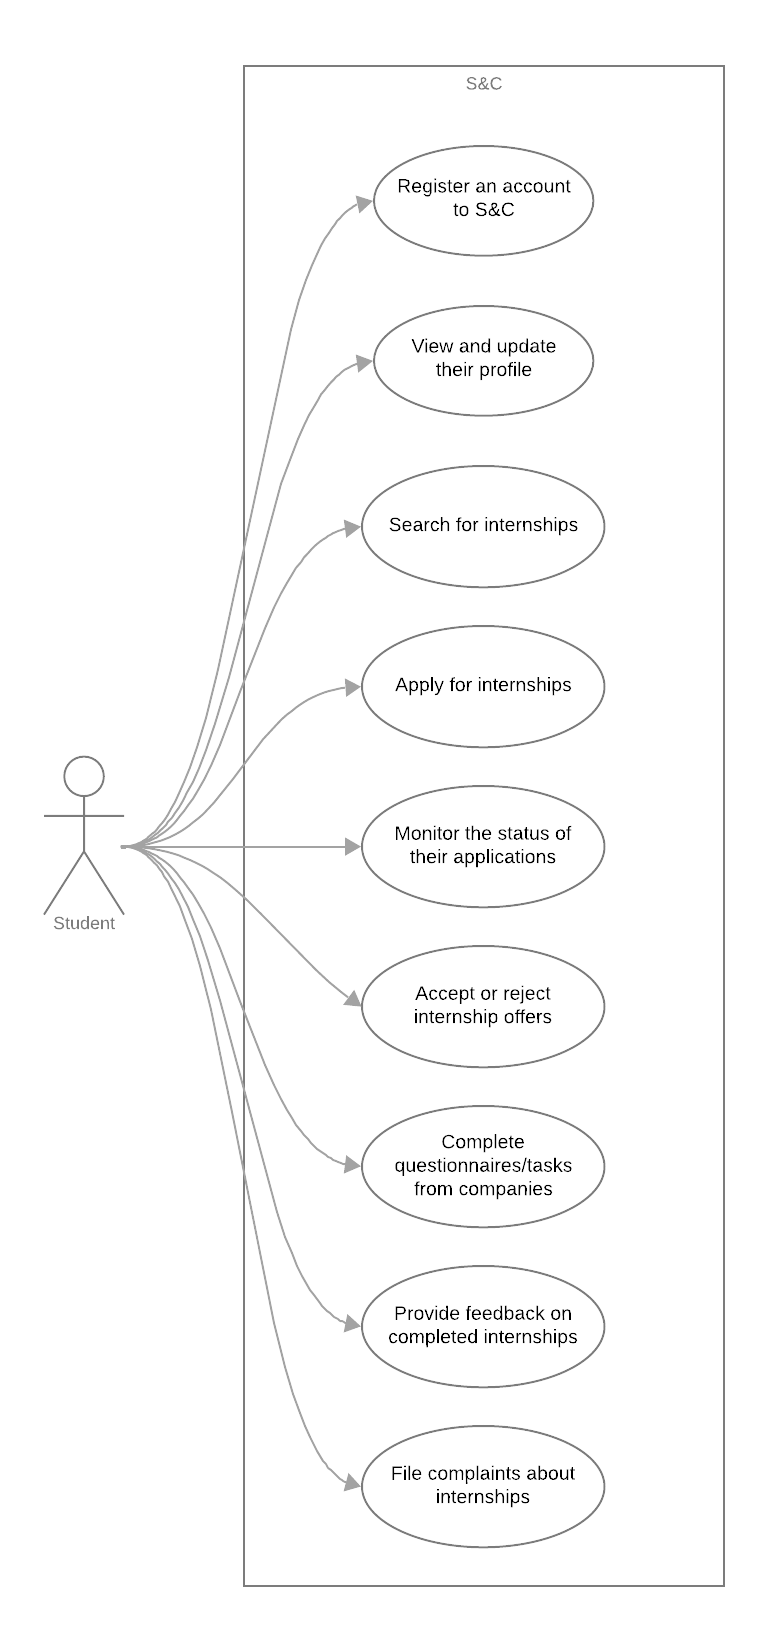
\includegraphics[width=0.6\linewidth]{UseCaseDiagrams/UC_Student.png}
        \caption{Use Cases Diagram for students.} 
        \label{fig:StudentUC}%
    \end{center}
\end{figure}

\begin{figure}[H]
    \begin{center}
        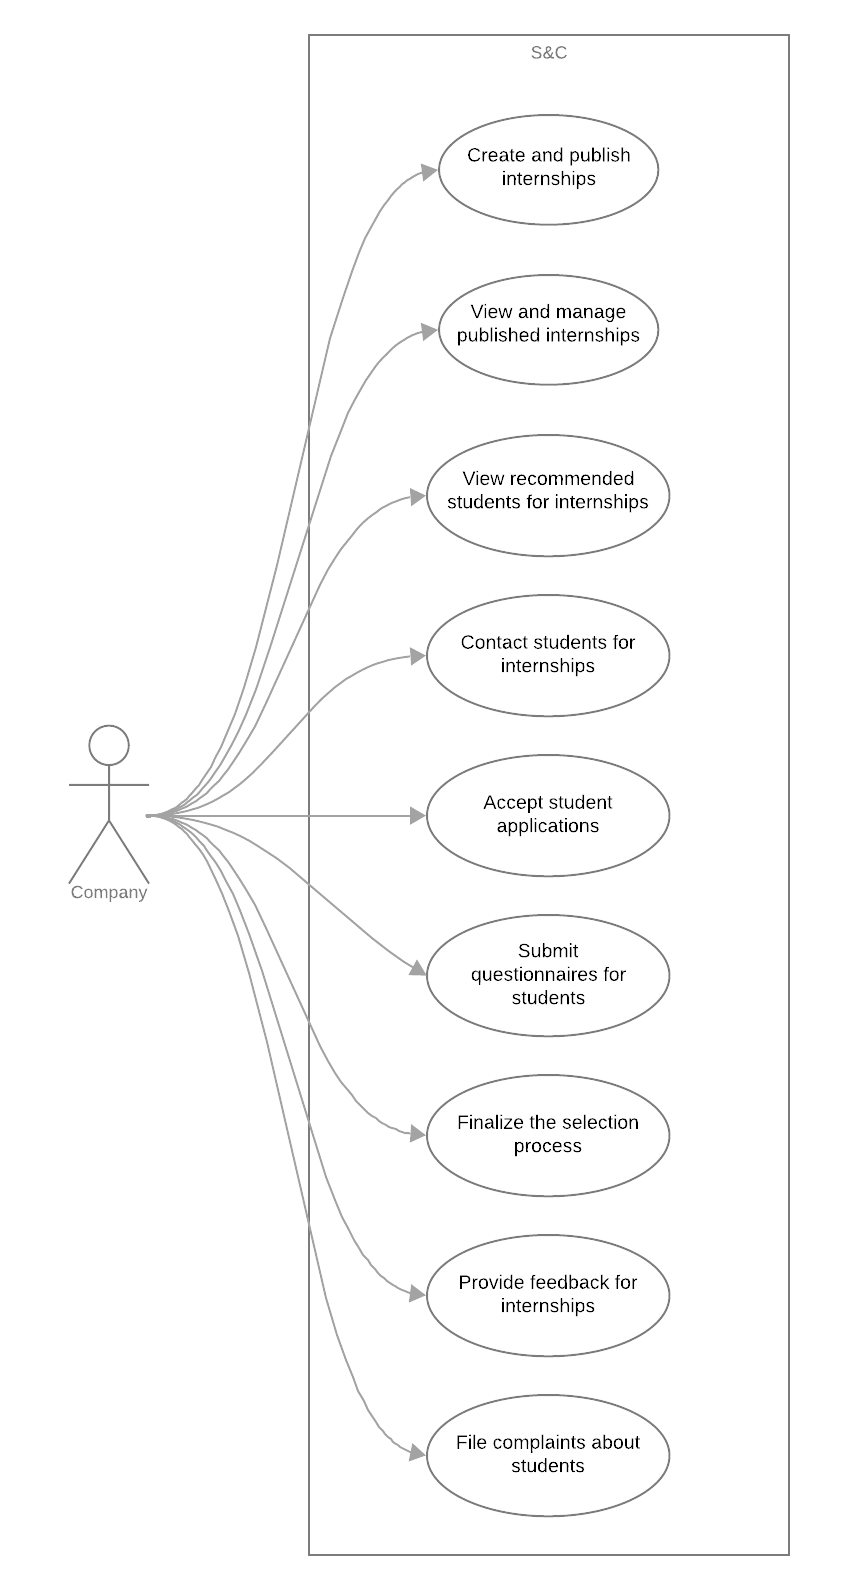
\includegraphics[width=0.8\linewidth]{UseCaseDiagrams/UC_Company.png}
        \caption{Use Cases Diagram for companies.} 
        \label{fig:CompanyUC}%
    \end{center}
\end{figure}

\begin{figure}[H]
    \begin{center}
        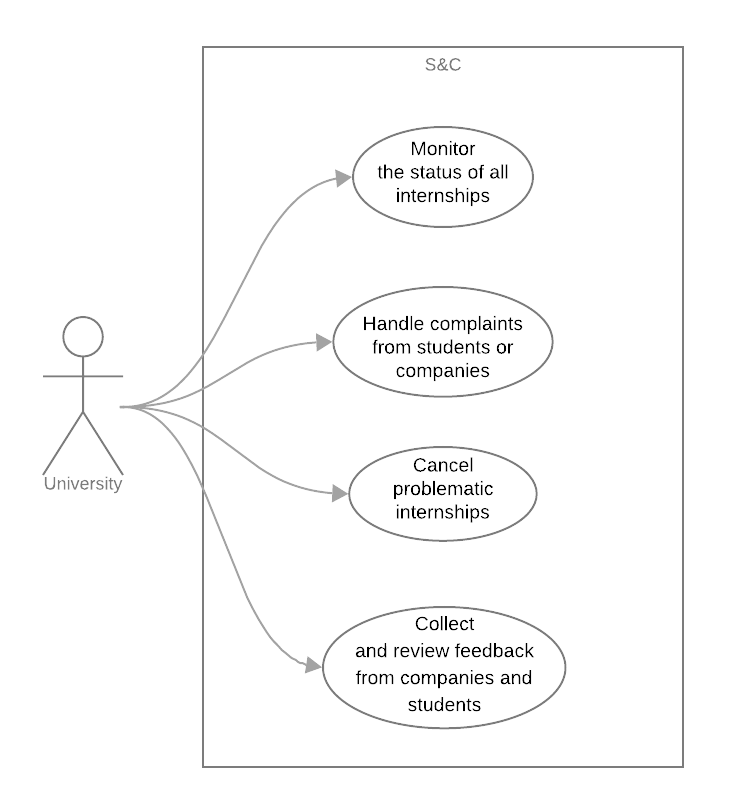
\includegraphics[width=0.6\linewidth]{UseCaseDiagrams/UC_University.png}
        \caption{Use Cases Diagram for universities.} 
        \label{fig:UniversityUC}%
    \end{center}
\end{figure}

\begin{figure}[H]
    \begin{center}
        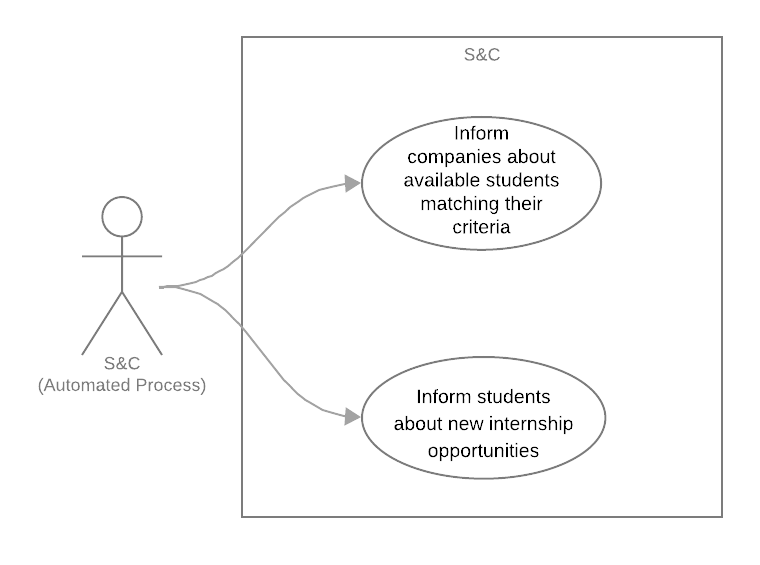
\includegraphics[width=0.6\linewidth]{UseCaseDiagrams/UC_SeC.png}
        \caption{Use Cases Diagram for S\&C.} 
        \label{fig:SeCUC}%
    \end{center}
\end{figure}

\newpage
\subsection{Use cases}
\label{subsec: use_cases}%
\newcounter{uc}
\setcounter{uc}{1}
\newcommand{\cuc}{\theuc\stepcounter{uc}}
In this section, they are explained and represented the main identified use cases.\\
There is a table with entry conditions, event flow, exit conditions and exception for each of them, and a sequence diagram that shows the messages exchanged between the entities and the called functions. \\


\subsubsection*{UC\cuc . Signup as ED}
\begin{center}
    \begin{longtable}{|l|p{0.75\linewidth}|}
        \hline
        \textbf{Actor}            & ED, eMail provider\\
        \hline
        \textbf{Entry conditions} & The ED is not already registered in CKB and has to search the CKB URL in the browser search bar \\
        \hline
        \textbf{Event Flow}       & 1 - CKB shows the login form.  \\
        & 2 - The ED clicks on “Create an Account” button.   \\
        & 3 - CKB shows the signup form.    \\
        & 4 - The ED inserts his name, surname, nickname, eMail and password in the form and also ticks on the “Signup as Educator” checkbox.  \\
        & 5 - The ED clicks on the “Register” button.  \\
        & 6 - CKB checks all the credentials.  \\
        & 7 - If credentials are correct CKB sends a confirmation eMail to the ED through the eMail provider.  \\
        & 8 - The ED clicks on the confirmation link.    \\
        \hline
        \textbf{Exit condition}   & CKB allows the ED to access to the CKB system. \\       
        \hline
        \textbf{Exceptions}       & \begin{itemize}
            \item The eMail address is already linked to an account. In this case an error message is shown and the ED is redirected to the profile creation settings.
            \item Invalid password if it is shorter than 8 characters, if it doesn’t have at least 1 number and/or 1 capital letter and/or a special character. In this case an error message is shown and the ED is redirected to the profile creation settings.
            \item  The nickname is already used. An error is shown and the ED is redirected to the profile creation settings.
        \end{itemize}\\
        \hline
        \caption{Signup as ED use case.}
        \label{tab:signup_as_ED_use_case}
    \end{longtable}
\end{center}

\begin{figure}[H]
    \begin{center}
        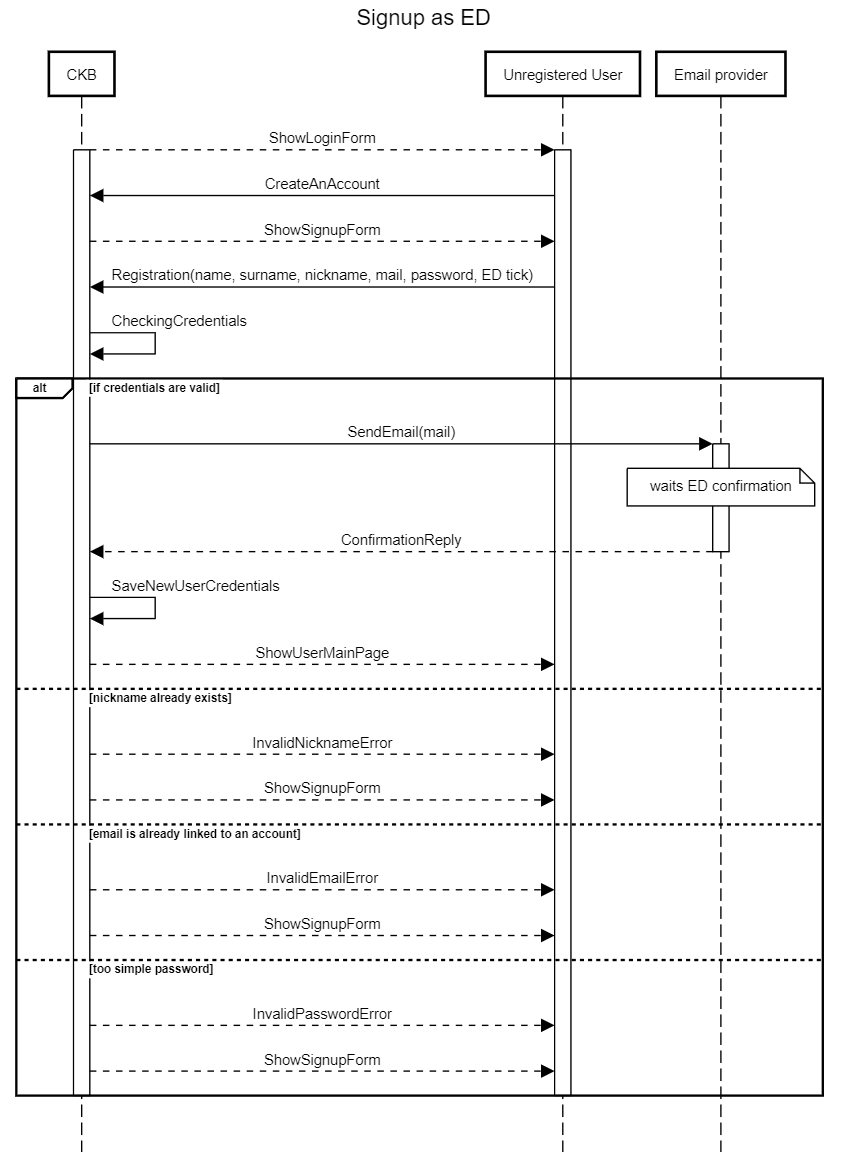
\includegraphics[width=1\linewidth]{SequenceDiagrams/ESEMPIO_Sequence.png}
        \caption{Signup as ED sequence diagram.}
        \label{fig:signup_as_ED_seqd}%
    \end{center}
\end{figure}

\newpage

\subsection{Requirement mapping}
\label{subsec:requirement_mapping}%
\textbf{G1 - Allow companies to post their internship opportunities.}
\begin{itemize}
    \item R2: The system shall allow Users to log in using their credentials.
    \item R4: The system shall enforce role-based access control to restrict access to specific functionalities based on the user type (ST, CP, UV).
    \item R5: The system shall allow CPs to post new internship opportunities, including position details, required skills, duration, and compensation.
    \item R20: The system shall maintain a database of all internships, applications, and evaluations.
\end{itemize}

\vspace{1.5cm}
\textbf{G2 - Allow students to search for available internships.}
\begin{itemize}
    \item R1: The system allows STs to register by providing personal information, email, and a password.
    \item R2: The system shall allow Users to log in using their credentials.
    \item R3: The system shall allow STs to edit their profiles, including personal details and contact information.
    \item R16: The system shall allow STs to search for internships using keywords, filters, or location.
    \item R17: The system shall recommend internships to STs based on their skills, preferences, and past applications.
\end{itemize}

\vspace{1.5cm}
\textbf{G3 - Notify students when an internship that might be of interest to them is posted.}
\begin{itemize}
    \item R12: The system shall send notifications to users for events such as application submissions, approvals, or rejections.
    \item R17: The system shall recommend internships to STs based on their skills, preferences, and past applications.
\end{itemize}

\vspace{1.5cm}
\textbf{G4 - Notify companies when a student matching their needs becomes available.}
\begin{itemize}
    \item R6: The system shall allow STs to apply for internships by submitting a CV and optional cover letter.
    \item R7: The system shall notify CPs when STs apply to an internship.
    \item R18: The system shall recommend STs to CPs for specific internships based on their skills, preferences, and past applications.
\end{itemize}

\vspace{1.5cm}
\textbf{G5 - Provide tools for both companies and students to manage the selection process.}
\begin{itemize}
    \item R2: The system shall allow Users to log in using their credentials.
    \item R8: The system shall allow CPs to review applications and schedule interviews with STs.
    \item R9: The system shall allow CPs to submit questionnaires to STs.
    \item R10: The system shall allow CPs to accept or reject applications and notify STs of the decision.
    \item R19: The system shall allow CPs to search for suitable STs based on their skills, academic background, and CVs.
\end{itemize}

\vspace{1.5cm}
\textbf{G6 - Collect feedback from students and companies to improve the matchmaking process.}
\begin{itemize}
    \item R2: The system shall allow Users to log in using their credentials.
    \item R13: The system shall allow CPs to track the progress of STs during the internship and provide regular feedback.
    \item R14: The system shall allow CPs to evaluate the performance of STs at the end of the internship.
    \item R15: The system shall allow UVs to review the feedback and evaluation provided by both CPs and STs.
\end{itemize}

\vspace{1.5cm}
\textbf{G7 - Provide suggestions for companies to improve internship descriptions and for students to improve their resumes.}
\begin{itemize}
    \item R4: The system shall enforce role-based access control to restrict access to specific functionalities based on the user type (ST, CP, UV).
    \item R17: The system shall recommend internships to STs based on their skills, preferences, and past applications.
    \item R18: The system shall recommend STs to CPs for specific internships based on their skills, preferences, and past applications.
\end{itemize}

\vspace{1.5cm}
\textbf{G8 - Allow all parties to monitor the status of the matchmaking process and the assigned internship.}
\begin{itemize}
    \item R2: The system shall allow Users to log in using their credentials.
    \item R13: The system shall allow CPs to track the progress of STs during the internship and provide regular feedback.
    \item R20: The system shall maintain a database of all internships, applications, and evaluations.
\end{itemize}

\vspace{1.5cm}
\textbf{G9 - Allow universities to monitor internships and handle any problems.}
\begin{itemize}
    \item R2: The system shall allow Users to log in using their credentials.
    \item R11: The system shall allow UVs to manage their students and monitor their activity.
    \item R12: The system shall send notifications to users for events such as application submissions, approvals, or rejections.
    \item R15: The system shall allow UVs to review the feedback and evaluation provided by both CPs and STs.
\end{itemize}

\vspace{2cm}
\newcounter{rtt}
\setcounter{rtt}{1}
\newcommand{\crt} {\thertt\stepcounter{rtt}}
\begin{center}
     \begin{longtable}{|l|c|c|c|c|c|c|c|c|c|}
    \hline
    \textbf{Requirements} & \textbf{G1} & \textbf{G2} & \textbf{G3} & \textbf{G4} & \textbf{G5} & \textbf{G6} & \textbf{G7} & \textbf{G8} & \textbf{G9}\\ \hline
    R1 &  & \checkmark  &  &  &  &  &  &  &  \\ \hline
    R2 & \checkmark & \checkmark & & & \checkmark & \checkmark & & \checkmark & \checkmark \\ \hline
    R3 &  & \checkmark &  &  &  &  &  &  &  \\ \hline
    R4 & \checkmark &  &  &  &  &  & \checkmark &  &  \\ \hline
    R5 & \checkmark &  &  &  &  &  &  &  &  \\ \hline
    R6 &  &  &  & \checkmark &  &  &  &  &  \\ \hline
    R7 &  &  &  & \checkmark &  &  &  &  &  \\ \hline
    R8 &  &  &  &  & \checkmark &  &  &  &  \\ \hline
    R9 &  &  &  &  & \checkmark &  &  &  &  \\ \hline
    R10 &  &  &  &  & \checkmark &  &  &  &  \\ \hline
    R11 &  &  &  &  &  &  &  &  & \checkmark \\ \hline
    R12 &  &  & \checkmark &  &  &  &  &  & \checkmark \\ \hline
    R13 &  &  &  &  &  & \checkmark &  & \checkmark &  \\ \hline
    R14 &  &  &  &  &  & \checkmark &  &  &  \\ \hline
    R15 &  &  &  &  &  & \checkmark &  &  & \checkmark \\ \hline
    R16 &  & \checkmark &  &  &  &  &  &  &  \\ \hline
    R17 &  & \checkmark & \checkmark &  &  &  & \checkmark &  &  \\ \hline
    R18 &  &  &  & \checkmark &  &  & \checkmark &  &  \\ \hline
    R19 &  &  &  &  & \checkmark &  &  &  &  \\ \hline
    R20 & \checkmark &  &  &  &  &  &  & \checkmark &  \\ \hline
\caption{Traceability Matrix for Goals and Requirements}
\label{tab:traceability}
\end{longtable}
\end{center}

\section{Performance requirements}
\label{sec:performance_requirements}%

\paragraph{Number of Concurrent Users:}
The S\&C system is expected to handle a significant number of concurrent users, based on research from similar platforms. The system architecture will be designed to scale dynamically to ensure consistent performance under heavy loads. Load testing will be conducted during development to verify this capacity.

\paragraph{Data Storage and Management:}
The system must efficiently handle large volumes of data, including:
\begin{itemize}
    \item Personal information of Students (ST) and Companies (CP).
    \item Records of all Internship Listings, Applications, and Interactions between users.
    \item Historical data for old internship offers. This information will remain stored indefinitely to allow CPs to review their previous postings and applicants.
\end{itemize}
To ensure scalability, a database management system with high throughput will be used. Additionally, data archiving strategies will be implemented to optimize storage for historical data without affecting performance.

\paragraph{Response Time:}
Actions executed directly by the S\&C system must have a response time of less than 500 milliseconds in normal conditions. Operations involving external services such as email systems may experience delays depending on the response times of those services. In case of a slow internet connection on the user's side, performance might degrade..

\section{Design constraints}
\label{sec:design_constraints}%

\subsection{Standard compliance}
\label{subsec:standard compliance}%%
The system must be compliant with the following standards and regulations:
\begin{itemize}
    \item EU's GDPR (General Data Protection Regulation), a set of regulations that is designed in order to protect the personal data, the privacy and security of the EU's citizens.
    \item WCAG (Web Content Accessibility Guidelines): The user interface will follow WCAG 2.1 Level AA guidelines to ensure accessibility for users with disabilities. This includes providing text alternatives for non-text content, keyboard navigation support, and ensuring sufficient contrast in the UI design.
\end{itemize}

\subsection{Hardware limitations}
\label{subsec:hardware_limitations}%
The platform is designed as a web application and does not require specific hardware. The users must have a device with a modern web browser and a reliable internet connection with a minimum recommended speed of 2 Mbps to ensure a smooth experience.

\section{Software system attributes}
\label{sec:software_system_attributes}%

\subsection{Reliability}
\label{subsec:reliability}%
The system has to be reliable because it will have to run continuously for a long period
of time. To ensure this feature the platform must have:
\begin{itemize}
    \item Some sort of replication and consistency policy to avoid system crash.
    \item Offline backups of the system in multiple locations to recover information after data loss or catastrophic failures.
    \item A monitoring system that alerts administrators in case of problems.
\end{itemize}

\subsection{Availability}
\label{subsec:availability}%
The most important attribute that the system has to provide is the availability. The
system should have an availability of 99\% to not interfere with users’ activities. To achieve this:
\begin{itemize}
    \item Replication policies must be implemented and a single point of failure should be avoided.
    \item Maintenance should be scheduled during low traffic periods (e.g., late-night) and notify users in advance.
    \item The recommendation algorithm should be optimized to run primarily during low-load hours, minimizing the impact on system performance during peak usage.
\end{itemize}

\subsection{Security}
\label{subsec:security}%
To protect user data and system integrity. The system must implement:
\begin{itemize}
    \item Authentication and authorization mechanisms, ensuring that only verified users can access the platform and perform actions based on their roles.
    \item Encryption for all sensitive data and communications between the client and server.
    \item Protection against common web vulnerabilities.
    \item Logging and monitoring of suspicious activities, such as repeated failed login attempts or unauthorized access attempts.
\end{itemize}

\subsection{Maintainability}
\label{subsec:maintainability}%
To ensure maintainability of the system the following actions are required:
\begin{itemize}
    \item Fllow modular and reusable design principles, ensuring that individual components can be updated or replaced without affecting the entire system.
    \item The code has to be well documented.
    \item A testing routine has to be provided and it has to cover at least 75\% of the entire code excluding the UI code.
\end{itemize}

\subsection{Portability}
\label{subsec:portability}%
The system should be portable, ensuring access across different platforms and environments.
\begin{itemize}
    \item Client-side the platform must be compatible with modern web browsers on both desktop and mobile devices.
    \item Server-side the backend should be deployable on multiple hosting environments, such as on-premises servers or cloud platforms without significant modifications. To ease this, use of containerization technologies is suggested.
\end{itemize}